\begin{figure*}
\begin{center}
\bgroup 
 \def\arraystretch{0.2} 
 \setlength\tabcolsep{0.2pt}
\begin{tabular}{ccccc}
L1 & 1$\times$1 & 16$\times$16 & 70$\times$70 & 286$\times$286 \\ 
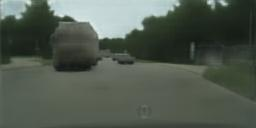
\includegraphics[width=0.2\linewidth]{figs/cityscapes_patchsize_variations_latex/L1_270.jpg} &
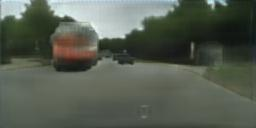
\includegraphics[width=0.2\linewidth]{figs/cityscapes_patchsize_variations_latex/0layers_270.jpg} &
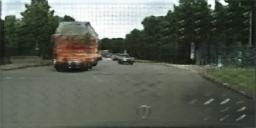
\includegraphics[width=0.2\linewidth]{figs/cityscapes_patchsize_variations_latex/1layers_270.jpg} &
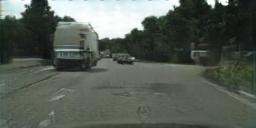
\includegraphics[width=0.2\linewidth]{figs/cityscapes_patchsize_variations_latex/L1cGAN_270.jpg} &
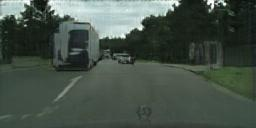
\includegraphics[width=0.2\linewidth]{figs/cityscapes_patchsize_variations_latex/5layers_270.jpg} %\\ 
%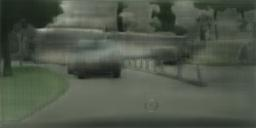
\includegraphics[width=0.2\linewidth]{figs/cityscapes_patchsize_variations_latex/L1_229.jpg} &
%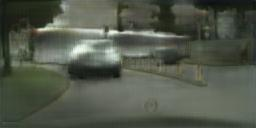
\includegraphics[width=0.2\linewidth]{figs/cityscapes_patchsize_variations_latex/0layers_229.jpg} &
%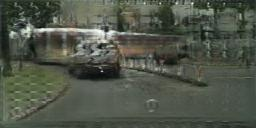
\includegraphics[width=0.2\linewidth]{figs/cityscapes_patchsize_variations_latex/1layers_229.jpg} &
%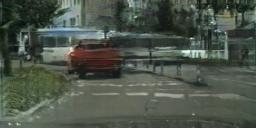
\includegraphics[width=0.2\linewidth]{figs/cityscapes_patchsize_variations_latex/L1cGAN_229.jpg} &
%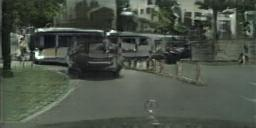
\includegraphics[width=0.2\linewidth]{figs/cityscapes_patchsize_variations_latex/6layers_229.jpg} \\ 
%\includegraphics[width=0.2\linewidth]{figs/facades2_patchsize_variations_latex/L1_83.jpg} &
%\includegraphics[width=0.2\linewidth]{figs/facades2_patchsize_variations_latex/0layers_83.jpg} &
%\includegraphics[width=0.2\linewidth]{figs/facades2_patchsize_variations_latex/1layers_83.jpg} &
%\includegraphics[width=0.2\linewidth]{figs/facades2_patchsize_variations_latex/L1cGAN_83.jpg} &
%\includegraphics[width=0.2\linewidth]{figs/facades2_patchsize_variations_latex/6layers_83.jpg}
\end{tabular} \egroup 
\end{center}
\vspace{-0.1in}
\caption{Patch size variations. Uncertainty in the output manifests itself differently for different loss functions. Uncertain regions become blurry and desaturated under L1. The 1x1 PixelGAN encourages greater color diversity but has no effect on spatial statistics. The 16x16 PatchGAN creates locally sharp results, but also leads to tiling artifacts beyond the scale it can observe. The 70$\times$70 PatchGAN forces outputs that are sharp, even if incorrect, in both the spatial and spectral (colorfulness) dimensions. The full 286$\times$286 ImageGAN produces results that are visually similar to the 70$\times$70 PatchGAN, but somewhat lower quality according to our FCN-score metric (Table \ref{tab:patchsize_variations}). Please see \texttt{https://phillipi.github.io/pix2pix/} for additional examples.}
\label{patchsize_variations_qualitative}
\vspace{-0.2in}
\end{figure*}